\appendix
\chapter{ROBE DA SWMM}
\label{appendix:SWMM}
%
\begin{figure}[htbp]
    \centering
    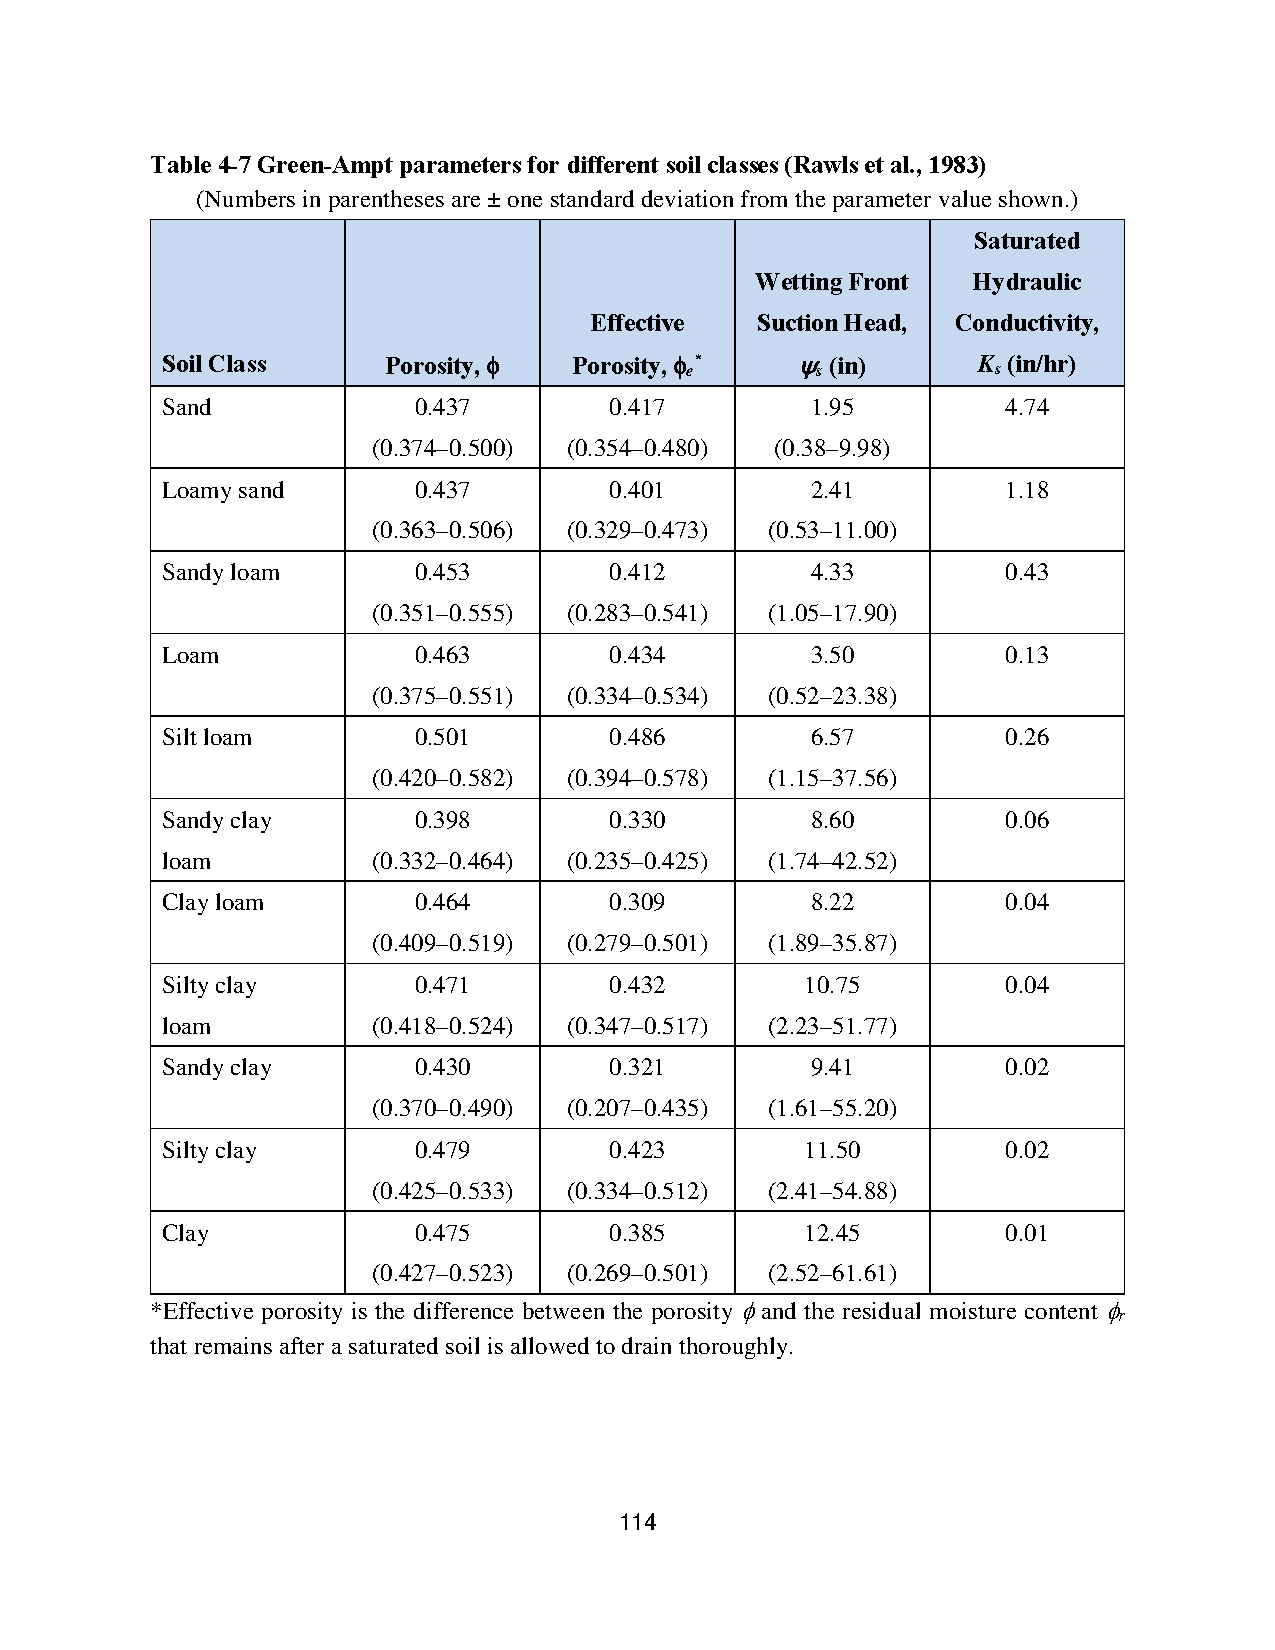
\includegraphics[trim=2.5cm 4.5cm 2.5cm 3.6cm,clip,width=\textwidth]{IMG/table4-7_Ks.pdf} 
    \caption[Tabella 4.7 di SWMM]{Tabella 4.7 di SWMM Green-Ampt parameters for different soil classes (Rawls et al., 1983) (Numbers in parentheses are ± one standard deviation from the parameter value shown.)}
    \label{SWMM:tabella4-7}
\end{figure}

%\chapter{Rete di smaltimento delle acque meteoriche allo stato di progetto (con presenza della rete di drenaggio) - tutti i mancanti}
%\label{appendix:FasiIntermedie}
%\section{Progetto sbagliato}
%\section{Progetto con solo i LID}
%\TabellaDiametriCondotte{Diametri progetti conduct-mod LID. In verde sono indicati i valori che hanno subito una modifica rispetto al progetto senza LID}{tab:Diametri_conduct-mod-LID}{IMG/Diametri-conduct-mod-LID.tex}
%\TabellaVerificheLinkFLow{Progetto con aggiunta dei soli LID -- Verifiche di massima velocità, riempimento condotta e del criterio di autopulizia}{tab:LinkFlow_Verifiche-MOD-LID}{IMG/LinkFlow-Verifiche-MOD-LID.tex}
%\section{Progetto con vasche e lid rifatto dopo i lid}
%\section{Progetto con vasche e lid sistemato}

\chapter{Computo metrico}
